\section{Evaluation}

\begin{frame}{GPU Utilization}
    % \todomark{Show profiler utilization}
    %     % TODO may need to use event synch to get profiler to look better for utilization
    % % https://on-demand.gputechconf.com/gtc/2014/presentations/S4158-cuda-streams-best-practices-common-pitfalls.pdf
    % % page 64
    
    \begin{wideitemize}
        \item GPU Utilization is close to 100\% where possible.
    
        \item At tick boundaries some bubbles appear as the CPU calculates the next $\delta{t}$.
    
        \item When visualizing, the Vulkan work hides this.
    \end{wideitemize}

    \vfill\null
    \begin{minipage}{0.49\textwidth}
        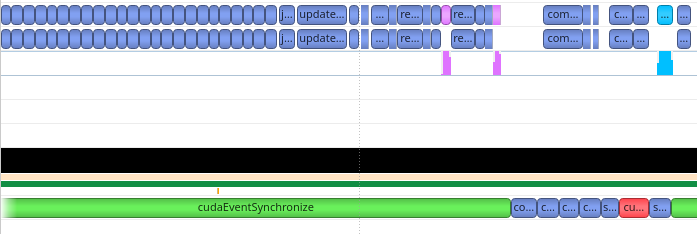
\includegraphics[width=\textwidth]{Presentation/images/sim_tick_edge.png}
        \begin{center}
            Tick Boundary
        \end{center}
    \end{minipage}\hfill%
    \begin{minipage}{0.49\textwidth}
        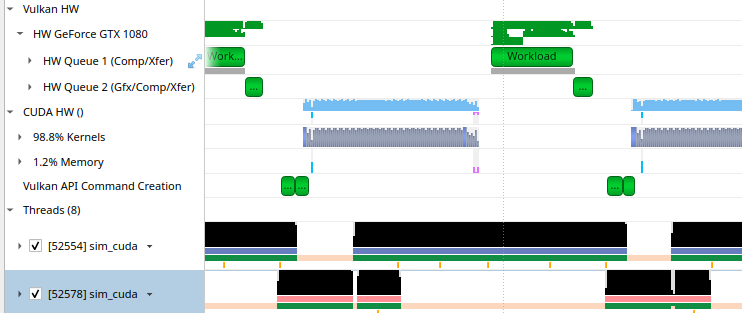
\includegraphics[width=\textwidth]{Presentation/images/final_pipeline_implementation.png}
        \begin{center}
            {Overall Visualization Pipeline}
        \end{center}
    \end{minipage}%\hfill%
    % \begin{minipage}{0.3\textwidth}
    
    % \end{minipage}
\end{frame}

\begin{frame}{Speed}
    % \todomark{Show graph of speed vs size for headless}
    % Speedup increases with longer running times for DETAILED ONLY
    % Speedup for ACA is constant w.r.t. accuracy
    % Speedup for large decreases w.r.t accuracy
    % Mean speedup at 2.3x vs. adapted ACA
    % ALL SPEEDUPS WITHIN [1.76, 2.77]
    
    \begin{wideitemize}
        \item Simulates the original CS257 input 2.47-2.86x faster than the original code.
        \item Visualization takes ~1.35ms per frame (740 FPS) at highest iteration count $N = 1000$
        % \footnote{When simulating at 120Hz. When simulating on every frame hits 170 FPS.}
        \item Individual visualization features are quick, and combined take less time than the simulation.\footnote{All points measured here in worst-case: with auto-range on where possible, and with maximum particles onscreen.}
    \end{wideitemize}
    
    \vfill\null
    
    \makebox[\textwidth][c]{
    {\renewcommand{\arraystretch}{1.5}%
    \begin{tabular}{|r|S[table-format=1.2,retain-explicit-plus]|S[table-format=1.2,retain-explicit-plus]|S[table-format=1.2,retain-explicit-plus]|S[table-format=1.2,retain-explicit-plus]|S[table-format=1.2,retain-explicit-plus]|}
    \hline
        & {Base Frame} & {with Sim} & {Scalar Quantity} & {Vector Field} & {Particles} \\ 
    \hline
        Mean Time (\si{\milli\second}) & 0.30 & 1.18 & 0.39 & 0.46 & 0.42 \\
        $\triangle$ from base (\si{\milli\second}) & {-} & +0.88 & +0.09 & +0.16 & +0.12 \\ 
    \hline
    \end{tabular}
    }
    }
    % \todomark{FPS above 120 for both normal and detailed profiles}
    % \todomark{Show approx time taken for each viz feature}
\end{frame}

\begin{frame}{Difference vs. Original}
    % \todomark{Created a tool to check accuracy against expected data}
    % \todomark{Using the same simulation profile (same iteration count etc.) got within 1E-11}
    \begin{wideitemize}
        \item The program contains a comparison tool for checking similarity.
    
        \item Simulating the original CS257 test has a mean square error of $10^{-14}$ for velocities, and $10^{-9}$ for pressure. 
    
        \item As iteration count and simulation time increases, the error becomes larger.
        \item Multiple potential causes in algorithm and implementation, but haven't researched further.
    \end{wideitemize}
    
    \vfill\null
    
    \makebox[\textwidth][c]{
    {\renewcommand{\arraystretch}{1.5}%
    % \begin{table}[t]
    %     \centering
        \begin{tabular}{|r|c|c|c|c|}
        \hline
            N & {100} & {200} & {300} & {1000} \\ 
        \hline
            Velocity MSE (u,v) & $10^{-14}$ & $10^{-14}$ & $10^{-14}$ & $10^{-14}$ \\
            Pressure MSE (p) & $10^{-9}$ & $10^{-8}$ & $10^{-7}$ & $10^{-6}$ \\
        \hline
        \end{tabular}
    % \end{table}
    }
    }
    \begin{center}
        Mean Square Error for original CS257 input data, simulated for \SI{10}{\second}
    \end{center}
\end{frame}

% Simulation is fast
% - inherent speedup moving from CPU to GPU
% - easy to get an accurate version working on CUDA
% - but wasn't a one/done process - needed to be aware of CUDA best practices and features to get speedups.
% - in ACA case and high-res case runs faster than real-time, faster than CPU version
% - but very dependent on simulation inputs.

% Simulation is accurate
% - results are close to ACA code
% - some differences because CUDA version doesn't use double-precision arithmetic, and uses FMAs more than ACA


% Visualization is fast
% - Particle sim and quantity-by-scalar elements add X time
% - Vector-quantity is oddly slow
% - 